\documentclass[tikz]{standalone}
\usepackage{amsmath}
\usepackage{tikz}

\begin{document}

\begin{center}
\begin{figure}[h!]
\centering
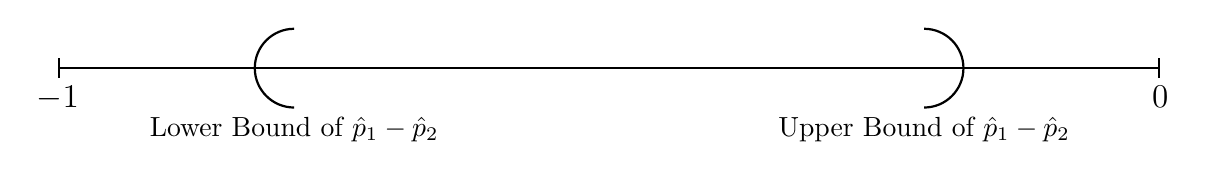
\begin{tikzpicture}
  \draw[|-|, thick] (-7,0) -- (7,0);
  \draw[thick] (-4,-0.5) arc (270:90:0.5);
  \node[below] at (-4,-0.5) {Lower Bound of $\hat{p}_1 - \hat{p}_2$};
  \draw[thick] (4,0.5) arc (90:-90:0.5);
  \node[below] at (4,-0.5) {Upper Bound of $\hat{p}_1 - \hat{p}_2$};
  \node[below] at (7, -0.1) {\large$0$};
  \node[below] at (-7, -0.1) {\large$-1$};
\end{tikzpicture}
\caption{Visualization of the case when $p_1 < p_2$}
\end{figure}
\end{center}

\end{document}